% vim: spell spelllang=en_gb
\chapter{Methods}

This section discusses and motivates the methods used in the project. Figure \ref{fig:flow_chart}
shows a flow chart of the steps for the pipeline (an enlarged and ma ore detailed copy is available in
Figure \ref{fig:flow_chart_big} of appendix \ref{appendix:raw}). The pipeline consists of the
following steps: Data collection, text classification, location extraction, and visualization.
Python is the primary programming language used for the project because of the rich ecosystem
surrounding it, especially when it comes to data science-related tasks. The code base is available
on a GitHub
repository\footnote{https://github.com/YasserKa/Classification-and-visualization-of-natural-disasters-using-Twitter}
accompanied with a \texttt{README.md} containing instructions to set up the environment and run the
project.

\begin{figure}[H]
\begin{center}
  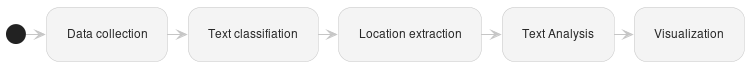
\includegraphics[width=\columnwidth]{./images/pipeline_concise.png}
\end{center}
\caption{Flow chart for the pipeline}
\label{fig:flow_chart}
\end{figure}

\section{Data Collection}

Finding a good quality data source is the first step to having a lean start for most research
questions. The pipeline trains an \ac{ML} classifier using three manually labelled datasets. Two of
them are crowdsourced datasets provided by Crisilext6; the tweets are from the 2013 flood events in
Alberta\footnote{https://en.wikipedia.org/wiki/2013\_Alberta\_floods} and
Queensland\footnote{https://en.wikipedia.org/wiki/Cyclone\_Oswald}, and there are around 10,000
records for each one with the tweet's ID, tweet's text, and a label about the relevance of the tweet
regarding the event. The third dataset is about some flood events in Sweden, spanning between 2015
and 2021; it contains 4899 tweets, mostly in the Swedish language, with attributes presented in
Table~\ref{tab:dataset_attr}. The text and metadata of the tweets are extracted from Twitter's API
using the IDs. The trained model performance is verified using tweets extracted from the API using
Tweepy\footnote{https://docs.tweepy.org/en/latest/index.html}, a python library for accessing
Twitter API. Figure~\ref{fig:flow_chart_data_collection_text_classification} shows both the source
and usage of the data in the pipeline.
\begin{figure}[H]
\begin{center}
  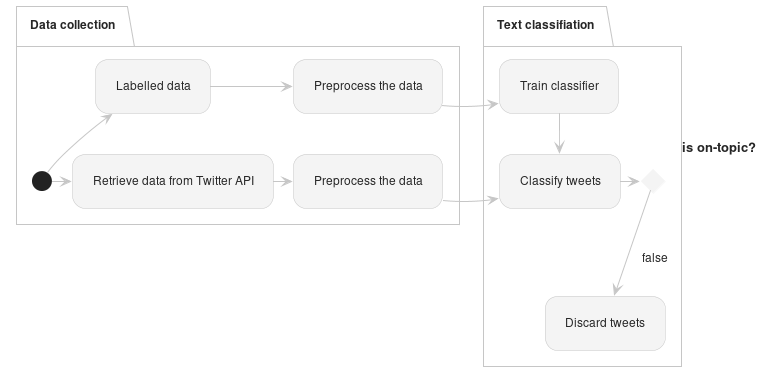
\includegraphics[width=\columnwidth]{./images/data_collection_text_classification.png}
\end{center}
\caption{Data collection and text classification steps of the pipeline}
\label{fig:flow_chart_data_collection_text_classification}
\end{figure}


\begin{table}
  \center
  \begin{tabular}{|l|l|l|}
    \hline
    Field & Type & Description \\
    \hline
    ID & Int & ID of the tweet\\
    \hline
    On Topic  & Bool & Text discusses an event \\
    \hline
    Informative sarcastic  & Bool & Text contains relevant information about the event \\
    \hline
    Contains IMPACT info & Bool & Text discusses the impact of the event \\
    \hline
    Explicit location & Bool & Text mentions the location of the event \\
    \hline
  \end{tabular}
  \caption{Dataset attributes}
  \label{tab:dataset_attr}
\end{table}

After retrieving the data, they are pre-processed to prepare them for the upcoming tasks, such as training an
\ac{ML} algorithm, text analysis, and visualization.  Parts of text that don't contribute to the
context are removed: \ac{URL}s, emojis, mentions, hashtag signs, numbers, new lines, punctuation,
and stopwords (provided by spaCy\footnote{https://spacy.io/}, an \ac{NLP} python library).
Afterwards, duplicate tweets, tweets containing no text, and retweets are discarded from the
dataset. The trained model requires the text to be in the English language, and since Sweden
is the focus of the research, most of the text is in Swedish; thus, the text is translated to
English using google translate\footnote{https://translate.google.com/} by a python library wrapper
deep-translate\footnote{https://deep-translator.readthedocs.io/en/latest/}. 

Data needs to be stored and managed to accommodate policies and regulations. Twitter's developer
policy\footnote{https://developer.twitter.com/en/developer-terms/policy} has a content
redistribution section stating that only the IDs of the tweets can be shared online. Thus, the
tweets can't be available publicly on such as GitHub, the service that hosts the publicly available
code base. To this end, the data is stored after each step on google drive using
\ac{DVC}'s\footnote{https://dvc.org/doc} data management capabilities.


Twitter's API provides an extensive list of information about the
tweets\footnote{https://developer.twitter.com/en/docs/twitter-api/data-dictionary/object-model/tweet}.
It shares the engagement metrics of the tweet, including like count, reply count, and retweet count;
as well as, an \ac{NLP} analysis of its own, such as the language used, and entities parsed from the
text. Table~\ref{tab:tweet_attr} shows the tweet's attributes used in this project for the following reasons: the id to
generate the \ac{URL} of the tweet, the text for \ac{NLP} tasks, the created date for temporal
analysis, and the author id to reduce spam.

\begin{table}
  \center
  \begin{tabular}{|l|l|l|}
    \hline
    Attribute & Type & Description \\
    \hline
    id & Int & The unique identifier of the requested Tweet \\
    \hline
    text & Str & The actual UTF-8 text of the Tweet \\
    \hline
    created at & Date  & Creation time of the Tweet \\
    \hline
    author id & Str & The unique identifier of the tweet creator \\
    \hline
  \end{tabular}
  \caption{Tweet attributes used}
  \label{tab:tweet_attr}
\end{table}

\section{Text Classification}

This project uses the DistilBERT transformer\cite{Sanh2019DistilBERTAD}, a variant of \ac{BERT}, for text
classification.  The main advantage of this model is that it achieves comparable performance to BERT
while being significantly smaller than BERT while being significantly smaller and more efficient. A
DistilBERT pre-trained model is provided by Hugging Face\footnote{https://huggingface.co/}, a
framework that provides a unified API for over more than 50 architectures, making it easier for
users to integrate \ac{NLP} models into their applications. The learning rate for the neural network
is $5\times e^{-5}$ with 100 warmup steps over four epochs using 90\% of the labelled tweets as
training data, 5\% as test data, and 5\% for validation. The text classification purpose is to
identify the tweets that discuss flood events, so the ``On Topic'' attribute of the dataset is used
as a label during training. 

Training the model locally takes a long time with the available resources, so the training is done
using Amazon SageMaker\footnote{https://aws.amazon.com/sagemaker/}, a service that covers tools to
build, train, and deploy \ac{ML} models. The data is uploaded to Amazon Simple Storage Service
(Amazon S3) to make it accessible for the Hugging Face training script that is executed in an
instance available in the cloud. After the training is complete, the fine-tuned model and the
evaluation metrics are downloaded. The evaluation metrics consists of the following:


\begin{itemize}
  \item Confusion matrix: a matrix showing the classifier's predictions for a labelled dataset
    corresponding to its actual values (Table~\ref{tab:confusion_matrix}).

    \begin{table}
      \center
      \bgroup
      \def\arraystretch{1.5}
      \begin{tabular}{@{}cc|cc@{}}
        \multicolumn{1}{c}{} &\multicolumn{1}{c}{} &\multicolumn{2}{c}{Predicted} \\ 
        \multicolumn{1}{c}{} & 
        \multicolumn{1}{c|}{} & 
        \multicolumn{1}{c}{Positive} & 
        \multicolumn{1}{c}{Negative} \\ 
        \cline{2-4}
        \multirow[c]{2}{*}{\rotatebox[origin=tr]{90}{Actual}}
                                     & Positive  & TP & FP   \\
                                     \cline{2-4}
                                     & Negative  & FN   & TN \\
                                     \cline{2-4}
      \end{tabular}
      \egroup
      \caption{Confusion matrix}
      \label{tab:confusion_matrix}
    \end{table}

  \item Accuracy: a fraction of the number of correctly classified instances (i.e., true positives
    and true negatives) among all instances (i.e., whole dataset) (equation~\ref{eq:accuracy}).
    \begin{equation}
      \text{Accuracy}=\frac{TN+TP}{TN+FN+TP+FP} 
      \label{eq:accuracy}
    \end{equation}
  \item Precision: a fraction of the number of correctly classified relevant instances (i.e., true
    positives) among the total number of instances classified as relevant (i.e., true positives and
    false positives) (equation~\ref{eq:precision}).
    \begin{equation}
      \text{Precision}=\frac{TP}{TP+FP} 
      \label{eq:precision}
    \end{equation}
  \item Recall: a fraction of the correctly classified relevant instances (i.e., true positives)
    among all relevant instances (i.e. true positives and false negatives) (equation~\ref{eq:recall}).
    \begin{equation}
      \text{Precision}=\frac{TP}{TP+FN} 
      \label{eq:recall}
    \end{equation}
  \item $\text{F}_1$ score: a harmonic mean of precision and recall (equation~\ref{eq:f1}).
    \begin{equation}
      \text{F}_1 =2.\frac{\text{Precision}.\text{Recall}}{\text{Precision}+\text{Recall}} 
      \label{eq:f1}
    \end{equation}
\end{itemize}


\section{Location Extraction}

The project uses a hybrid approach for geoparsing to extract locations. For toponym recognition, the
tokens representing locations are extracted using the KBLab/bert-base-swedish-cased-ner
model\footnote{https://huggingface.co/KBLab/bert-base-swedish-cased-ner}. The model is based on BERT
and fine-tuned for \ac{NER} using The Stockholm-Umeå Corpus, a collection of Swedish texts from the
1990s that consists of one million words. As for toponym resolution, the location tokens are
disambiguated using Nominatim and GeoNames geocoders through
Geopy\footnote{https://geopy.readthedocs.io/en/latest}, a Python client for several
popular geocoding web services. Nominatim retrieves different fields about the
location from OpenStreetMap. An example of the output is available in appendix
\ref{appendix:examples}.


The descriptions for the fields are available in the
documentation\footnote{https://nominatim.org/release-docs/develop/api/Output/}. The project uses
the lat, lon, and display\_name to represent the location on a map. In some cases, the text might
contain two locations, the one with the smaller bounding box (area of corner coordinates) is used,
which is, in most cases, a more specific place located in the bigger one (e.g. a street within a
municipality). The geocoder services provide the ability to limit the search of the locations
within a specific country. Since the project is limited to Sweden, the output can be limited using
this option, reducing the false positives that happen when different countries have places with
the same name. Tweets that don't contain location terms identifying a geographical
location are discarded as shown in Figure~\ref{fig:flow_chart_location_extraction}.

\begin{figure}[H]
  \begin{center}
    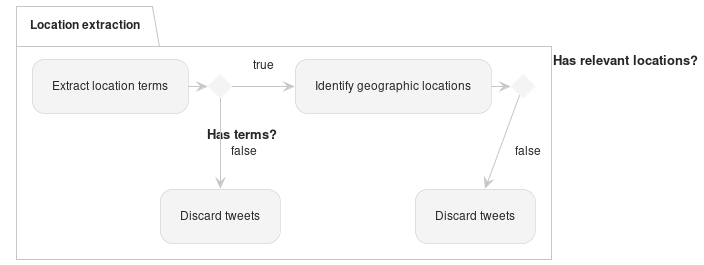
\includegraphics[width=\columnwidth]{./images/location_extraction.png}
  \end{center}
  \caption{Flow chart for the location extraction step of the pipeline}
  \label{fig:flow_chart_location_extraction}
\end{figure}


\section{Text analysis}

Further pre-processing is done on the dataset to prepare for text analysis tasks. Lemmatisation is
done on the text, using \ac{NLTK}\footnote{https://www.nltk.org/}, to reduce words to their lemmas.
Afterwards, Tokenisation is done on the corpus. Terms occurring in less than 20 documents or 5\% of
the documents are removed, as well as the terms mentioned in more than 75\% of the documents.
Bigrams that occur more than 20 times in the corpus are included, such as traffic jams, and climate
change. To reduce spam, tweets created by the same user who tweeted about the same location the past
week are discarded.

The text analysis used in the project are \ac{LDA} \cite{pritchardInferencePopulationStructure2000}
\cite{falushInferencePopulationStructure2003}, \ac{TF-IDF}, and
\ac{t-SNE}\cite{vandermaatenVisualizingHighDimensionalData2008}. \ac{LDA} is a topic modelling
method that generates topics (a set of terms) in a corpus and assigns the relevancy of each topic in
each document. The \ac{LDA} model is initialized and trained using Gensim \cite{rehurek_lrec},
where the number of discovered topics is adjustable in the visualization. The second text analysis
technique used is \ac{TF-IDF}, using scikit-learn\footnote{https://scikit-learn.org/stable/}, to
extract interesting terms by checking their average weight and frequency in the corpus. Lastly,
\ac{t-SNE} is a visualization method for high-dimensional data by reducing their dimensions to two
or three-dimensional maps. In this project, \ac{t-SNE} reduces the dimensions of a \ac{TF-IDF}
matrix generated from the corpus to 2-dimensional space and then presented on a scatter plot; the
points are clustered before applying \ac{t-SNE} using \ac{DBSCAN} with adjustable eps (maximum
distance between neighbours), and min\_samples (number of samples in a neighbourhood for the
point to be considered as a core point). \ac{t-SNE}, the generation of the \ac{TF-IDF} matrix, and
clustering are done using scikit-learn.

\section{Visualization}

Visualization is often placed at the end of the pipeline and might be the most important since it
brings meaning to the results, which can be interrupted by most audiences. Also, it's a direct way
to verify that the pipeline is working. The web application is made by
Dash\footnote{https://dash.plotly.com/} to create an interface for
Plotly\footnote{https://plotly.com/python/}'s visualizations. Dash Bootstrap
Components\footnote{https://dash-bootstrap-components.opensource.faculty.ai/} is used as well for
an easier way to use Bootstrap components for Plotly Dash, such as buttons, input, and tables.

There are several interactive graphs to enable spatial, temporal, and textual exploration of
tweets. The text, created time, location extracted, and other features of the selected tweets are
explored using a table. The identified locations are presented using clustered pointers on a map;
tweets selection can be done by clicking on the clusters or on a different level of regions
(counties or municipalities) that can be changed using radio items. The creation dates of tweets
are aggregated and plotted using a histogram; they are aggregated by day if the tweets span a
month or less; otherwise, by month. The results of \ac{LDA} and \ac{TF-IDF} are displayed in two
tables showing the frequency of the terms and their mean weights. The number of topics generated
by \ac{LDA} can be changed using a text input, and the tables can be regenerated after changing
the selected tweets by clicking a button. A scatter plot shows the \ac{t-SNE}'s 2-dimensional
space with \ac{DBSCAN}  clustering, where the clustering properties (eps and min samples) can be
adjusted by text inputs. Lastly, metadata about the interface is available: the total number
of tweets, the number of selected tweets, the oldest and newest tweet creation dates, the total
number of locations, the number of selected locations, and a list of locations' names. All
elements of the interface influence each other to some extent. Selecting tweets using the map,
histogram, or scatter plot will alter the view for the rest of the presentations by highlighting
only the selected tweets.

\section{Experiments}

The pipeline is applied to one week's worth of tweets starting from a date when a flood event happened
in Sweden and verified using the visualizations presented at the find step. The query is created by
experts at a workshop in \ac{SMHI} to extract tweets contain flood relevant terms in Swedish:

\begin{verbatim}
 "atmosfärisk flod" OR "hög vatten" OR åskskur
 OR regnskur OR dagvattensystem OR dränering OR "höga vågor"
 OR "höga flöden" OR dämmor
 OR snösmältning OR blött OR oväder OR stormflod OR vattenstånd
 OR vattennivå OR åskväder OR regnstorm"
 OR "mycket regn" OR "kraftig regn" OR översvämningsskador 
 OR översvämningar OR översvämning
\end{verbatim}
